
\chapter{Конструкторская часть}\label{Konstruct}
%\addcontentsline{toc}{chapter}{2 Конструкторская часть}

В данном разделе представлены схемы алгоритмов. Так же будут опи-
саны пользовательские структуры данных, приведены классы эквивалентности для тестирования реализуемого ПО.

\section{Схемы алгоритмов}\label{SchemaAlg}


\subsection{Схема последовательного алгоритма нахождения среднего арифметического матрицы}\label{SchemaPoslMatrixMultiply}

На рисунке \ref{ris:schemaposav} показана схема последовательного алгоритма умножения матриц.

\begin{figure}[H]
  \center{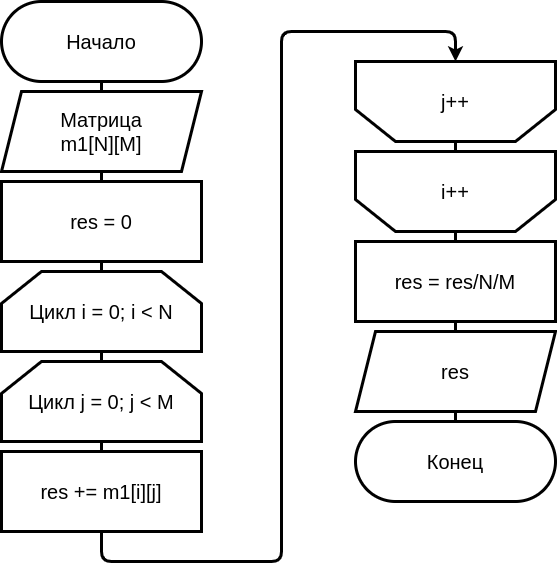
\includegraphics[scale=0.40]{l1.poslav}}
  \caption{Схема последовательного алгоритма}
  \label{ris:schemaposav}
\end{figure}

\subsection{Схема распараллеленного по строкам алгоритма нахождения среднего арифметического матрицы}\label{SchemaParRowMatrixMultiply}

На рисунке \ref{ris:schemaparrowav} показана схема распараллеленного по строкам алгоритма умножения матриц.

\begin{figure}[H]
  \center{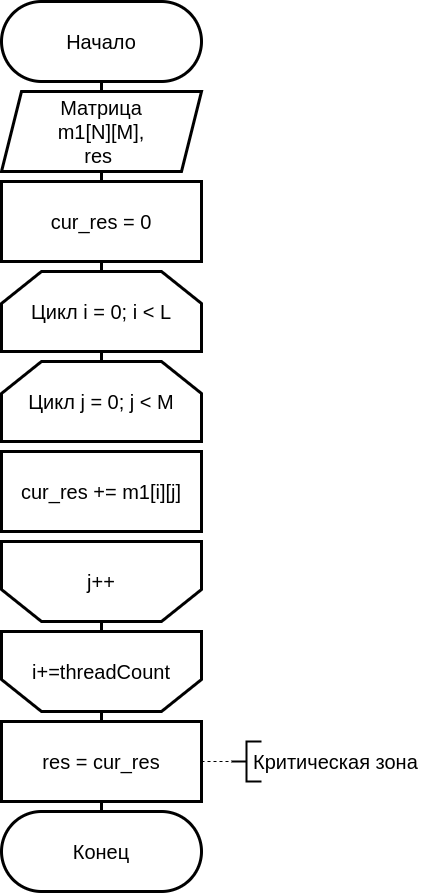
\includegraphics[scale=0.40]{l1.parrowav}}
  \caption{Схема распараллеленого по строкам алгоритма}
  \label{ris:schemaparrowav}
\end{figure}

\subsection{Схема распараллеленного по столбцам алгоритма нахождения среднего арифметического матрицы}\label{SchemaParColumnMatrixMultiply}

На рисунке \ref{ris:schemaparcolumnav} показана схема распараллеленного по столбцам алгоритма умножения матриц.

\begin{figure}[H]
  \center{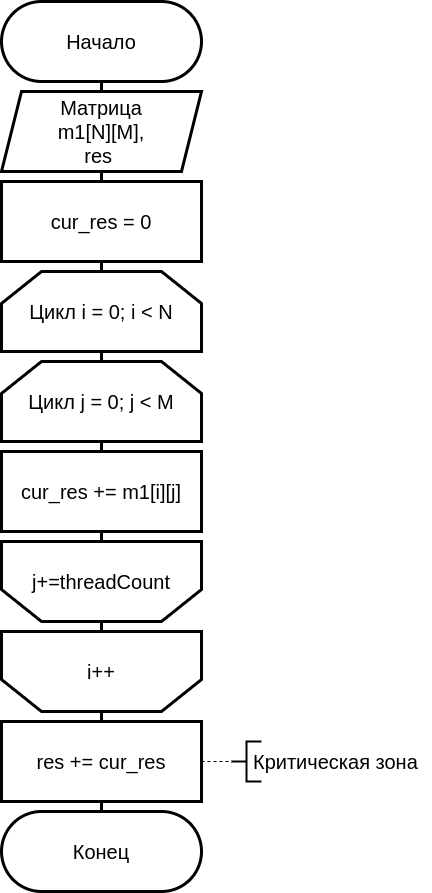
\includegraphics[scale=0.40]{l1.parcolumnav}}
  \caption{Схема распараллеленного по столбцам алгоритма}
  \label{ris:schemaparcolumnav}
\end{figure}

\subsection{Схема алгоритма управления потоками}\label{SchemaTheardControl}

На рисунке \ref{ris:schemacontrolthread} показана схема алгоритма управления потоками.

\begin{figure}[H]
  \center{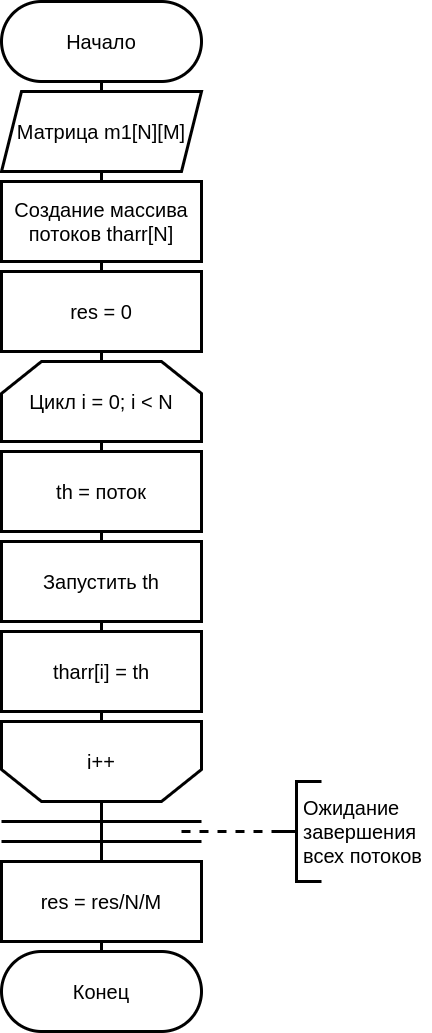
\includegraphics[scale=0.40]{l1.threadcontrol}}
  \caption{Схема алгоритма управления потоками}
  \label{ris:schemacontrolthread}
\end{figure}

%На рисунке \ref{ris:schemachoise} показана схема алгоритма сортировки выбором.

%\begin{figure}[H]
%  \center{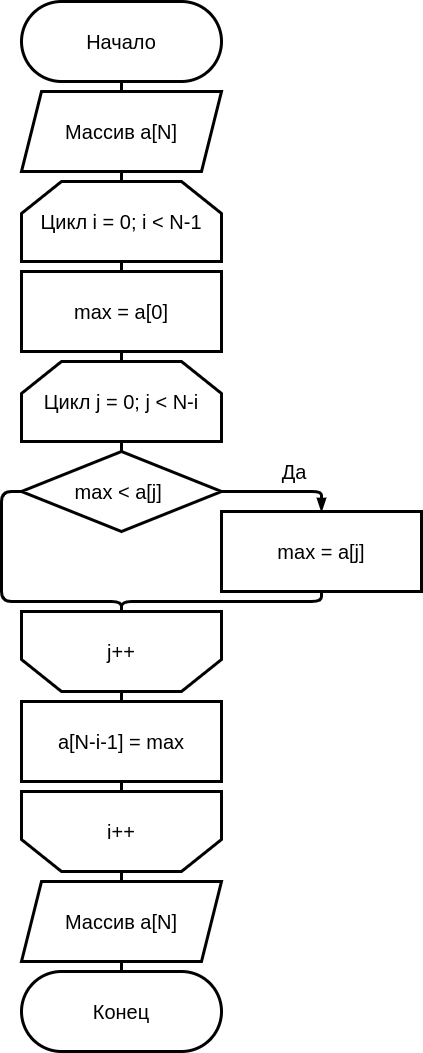
\includegraphics[scale=0.35]{l1.choise}}
%  \caption{Схема алгоритма сортировки выбором}
%  \label{ris:schemachoise}
%\end{figure}

%На рисунке \ref{ris:schemainsert} показана схема алгоритма сортировки вставками.

%\begin{figure}[H]
%  \center{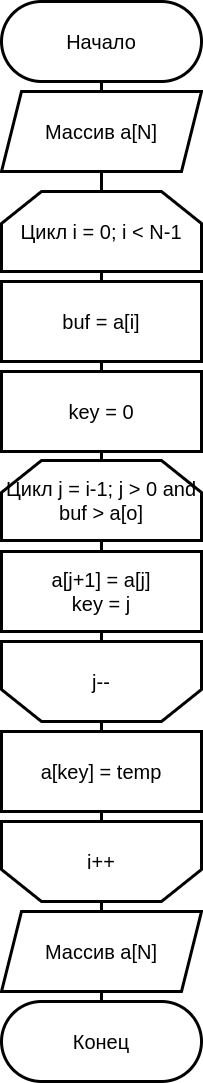
\includegraphics[scale=0.35]{l1.insert}}
%  \caption{Схема алгоритма сортировки вставками}
%  \label{ris:schemainsert}
%\end{figure}


\section{Структуры данных}\label{Structs}

При реализации приведенных алгоритмов потребуется тип данных: матрица.

\section{Тестирование}\label{Testing}


Для алгоритма умножения матриц можно выделить следующие классы эквивалентности:

\begin{enumerate}
    \item матрицы $ n\cdot m $ (где $n, m\in N$ );
    \item матрицы, где $ n = 0 $ или $ m = 0 $.
\end{enumerate}

%\subsection{Способы тестирования}\label{TestingMethods}

%При разработке программы удобно использовать следующие методы тестирования:

%\begin{enumerate}
%    \item Модульные тесты 
%    \item Функциональные тесты 
%\end{enumerate}

\section{Вывод конструкторской части}\label{KonstructResult}
На основе данных, полученных в аналитическом разделе, были построены схемы используемых алгоритмов,
выделены необходимые для реализации структуры данных и методы тестирования.

